\begin{figure}[h]
\centering
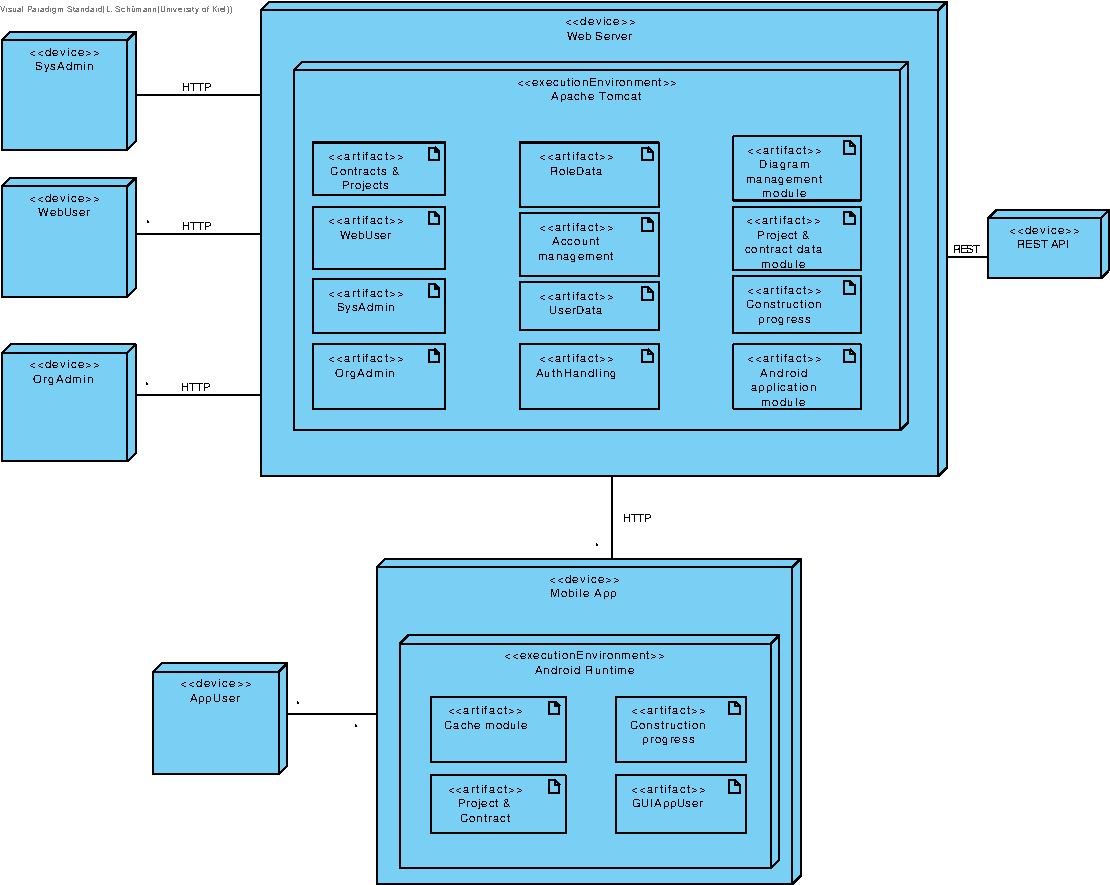
\includegraphics[width=\linewidth]{img/diagrams/Deployment-Diagram.pdf}
\caption{Verteilungsdiagramm}
\end{figure}
\clearpage
\noindent
Die Applikation (Mobile App) kommuniziert mit dem Webserver (Web Server) mittels HTTP,  um Projekt- und Vertragsdaten zu erhalten.  
Diese Schnittstelle ist unter dem Namen \textbf{App-API for data} jeweils im Komponentendiagramm von mobiler Applikation und Webserver eingezeichnet.
Hierf\"ur authentifiziert sich die Applikation per POST-Request,  indem sie ein Paar bestehend aus Benutzername und Passwort verschickt.  
Der Webserver antwortet mit einem JSON Web Token (JWT),  welches in den folgenden Nachrichten jeweils mitgesendet wird. 
Dieser Vorgang stellt sicher,  dass Ressourcen nur von Benutzern mit den entsprechenden Zugriffsrechten vom Server abgefragt werden k\"onnen.
Auf diese Weise bezieht die Applikation nun also Projekt- und Vertragsdaten  vom Webserver,  indem sie GET-Requests an den Server versendet.  
Dar\"uber hinaus erfolgt das Aktualisieren des Status einer Leistungsposition ebenfalls per POST-Request an den Server.








